%%%%%%%%%%%%%%%%%%%%%%%%%%%%%%%%%%%%%%%%%%%%%%%%%%%%%%%%%%%%%%%%%%%%%%
% Template for a UBC-compliant dissertation
% At the minimum, you will need to change the information found
% after the "Document meta-data"
%
%!TEX TS-program = pdflatex
%!TEX encoding = UTF-8 Unicode

%% The ubcdiss class provides several options:
%%   gpscopy (aka fogscopy)
%%       set parameters to exactly how GPS specifies
%%         * single-sided
%%         * page-numbering starts from title page
%%         * the lists of figures and tables have each entry prefixed
%%           with 'Figure' or 'Table'
%%       This can be tested by `\ifgpscopy ... \else ... \fi'
%%   10pt, 11pt, 12pt
%%       set default font size
%%   oneside, twoside
%%       whether to format for single-sided or double-sided printing
%%   balanced
%%       when double-sided, ensure page content is centred
%%       rather than slightly offset (the default)
%%   singlespacing, onehalfspacing, doublespacing
%%       set default inter-line text spacing; the ubcdiss class
%%       provides \textspacing to revert to this configured spacing
%%   draft
%%       disable more intensive processing, such as including
%%       graphics, etc.
%%

% For submission to GPS
\documentclass[gpscopy,onehalfspacing,11pt]{ubcdiss}
% For your own copies (looks nicer)
% \documentclass[balanced,twoside,11pt]{ubcdiss}

%%%%%%%%%%%%%%%%%%%%%%%%%%%%%%%%%%%%%%%%%%%%%%%%%%%%%%%%%%%%%%%%%%%%%%
%%%%%%%%%%%%%%%%%%%%%%%%%%%%%%%%%%%%%%%%%%%%%%%%%%%%%%%%%%%%%%%%%%%%%%
%%
%% FONTS:
%% 
%% The defaults below configures Times Roman for the serif font,
%% Helvetica for the sans serif font, and Courier for the
%% typewriter-style font.  Configuring fonts can be time
%% consuming; we recommend skipping to END FONTS!
%% 
%% If you're feeling brave, have lots of time, and wish to use one
%% your platform's native fonts, see the commented out bits below for
%% XeTeX/XeLaTeX.  This is not for the faint at heart. 
%% (And shouldn't you be writing? :-)
%%

%% NFSS font specification (New Font Selection Scheme)
\usepackage{times,mathptmx,courier}
\usepackage[scaled=.92]{helvet}

%% Math or theory people may want to include the handy AMS macros
\usepackage{amssymb} % for $\mathbb{R}$, Real R
%\usepackage{amsmath}
%\usepackage{amsfonts}

%% The pifont package provides access to the elements in the dingbat font.   
%% Use \ding{##} for a particular dingbat (see p7 of psnfss2e.pdf)
%%   Useful:
%%     51,52 different forms of a checkmark
%%     54,55,56 different forms of a cross (saltyre)
%%     172-181 are 1-10 in open circle (serif)
%%     182-191 are 1-10 black circle (serif)
%%     192-201 are 1-10 in open circle (sans serif)
%%     202-211 are 1-10 in black circle (sans serif)
%% \begin{dinglist}{##}\item... or dingautolist (which auto-increments)
%% to create a bullet list with the provided character.
\usepackage{pifont}

%%%%%%%%%%%%%%%%%%%%%%%%%%%%%%%%%%%%%%%%%%%%%%%%%%%%%%%%%%%%%%%%%%%%%%
%% Configure fonts for XeTeX / XeLaTeX using the fontspec package.
%% Be sure to check out the fontspec documentation.
%\usepackage{fontspec,xltxtra,xunicode}	% required
%\defaultfontfeatures{Mapping=tex-text}	% recommended
%% Minion Pro and Myriad Pro are shipped with some versions of
%% Adobe Reader.  Adobe representatives have commented that these
%% fonts can be used outside of Adobe Reader.
%\setromanfont[Numbers=OldStyle]{Minion Pro}
%\setsansfont[Numbers=OldStyle,Scale=MatchLowercase]{Myriad Pro}
%\setmonofont[Scale=MatchLowercase]{Andale Mono}

%% Other alternatives:
%\setromanfont[Mapping=tex-text]{Adobe Caslon}
%\setsansfont[Scale=MatchLowercase]{Gill Sans}
%\setsansfont[Scale=MatchLowercase,Mapping=tex-text]{Futura}
%\setmonofont[Scale=MatchLowercase]{Andale Mono}
%\newfontfamily{\SYM}[Scale=0.9]{Zapf Dingbats}
%% END FONTS
%%%%%%%%%%%%%%%%%%%%%%%%%%%%%%%%%%%%%%%%%%%%%%%%%%%%%%%%%%%%%%%%%%%%%%
%%%%%%%%%%%%%%%%%%%%%%%%%%%%%%%%%%%%%%%%%%%%%%%%%%%%%%%%%%%%%%%%%%%%%%



%%%%%%%%%%%%%%%%%%%%%%%%%%%%%%%%%%%%%%%%%%%%%%%%%%%%%%%%%%%%%%%%%%%%%%
%%%%%%%%%%%%%%%%%%%%%%%%%%%%%%%%%%%%%%%%%%%%%%%%%%%%%%%%%%%%%%%%%%%%%%
%%
%% Recommended packages
%%
\usepackage{checkend}	% better error messages on left-open environments
\usepackage{graphicx}	% for incorporating external images

%% booktabs: provides some special commands for typesetting tables as used
%% in excellent journals.  Ignore the examples in the Lamport book!
\usepackage{booktabs}

%% listings: useful support for including source code listings, with
%% optional special keyword formatting.  The \lstset{} causes
%% the text to be typeset in a smaller sans serif font, with
%% proportional spacing.
\usepackage{listings}
\lstset{basicstyle=\sffamily\scriptsize,showstringspaces=false,fontadjust}

%% The acronym package provides support for defining acronyms, providing
%% their expansion when first used, and building glossaries.  See the
%% example in glossary.tex and the example usage throughout the example
%% document.
%% NOTE: to use \MakeTextLowercase in the \acsfont command below,
%%   we *must* use the `nohyperlinks' option -- it causes errors with
%%   hyperref otherwise.  See Section 5.2 in the ``LaTeX 2e for Class
%%   and Package Writers Guide'' (clsguide.pdf) for details.
\usepackage[printonlyused,nohyperlinks]{acronym}
%% The ubcdiss.cls loads the `textcase' package which provides commands
%% for upper-casing and lower-casing text.  The following causes
%% the acronym package to typeset acronyms in small-caps
%% as recommended by Bringhurst.
\renewcommand{\acsfont}[1]{{\scshape \MakeTextLowercase{#1}}}

%% color: add support for expressing colour models.  Grey can be used
%% to great effect to emphasize other parts of a graphic or text.
%% For an excellent set of examples, see Tufte's "Visual Display of
%% Quantitative Information" or "Envisioning Information".
\usepackage{color}
\definecolor{greytext}{gray}{0.5}

%% comment: provides a new {comment} environment: all text inside the
%% environment is ignored.
%%   \begin{comment} ignored text ... \end{comment}
\usepackage{comment}

%% The natbib package provides more sophisticated citing commands
%% such as \citeauthor{} to provide the author names of a work,
%% \citet{} to produce an author-and-reference citation,
%% \citep{} to produce a parenthetical citation.
%% We use \citeeg{} to provide examples
\usepackage[numbers,sort&compress]{natbib}
\newcommand{\citeeg}[1]{\citep[e.g.,][]{#1}}

%% The titlesec package provides commands to vary how chapter and
%% section titles are typeset.  The following uses more compact
%% spacings above and below the title.  The titleformat that follow
%% ensure chapter/section titles are set in singlespace.
\usepackage[compact]{titlesec}
\titleformat*{\section}{\singlespacing\raggedright\bfseries\Large}
\titleformat*{\subsection}{\singlespacing\raggedright\bfseries\large}
\titleformat*{\subsubsection}{\singlespacing\raggedright\bfseries}
\titleformat*{\paragraph}{\singlespacing\raggedright\itshape}

%% The caption package provides support for varying how table and
%% figure captions are typeset.
\usepackage[format=hang,indention=-1cm,labelfont={bf},margin=1em]{caption}

%% url: for typesetting URLs and smart(er) hyphenation.
%% \url{http://...} 
\usepackage{url}
\urlstyle{sf}	% typeset urls in sans-serif


%%%%%%%%%%%%%%%%%%%%%%%%%%%%%%%%%%%%%%%%%%%%%%%%%%%%%%%%%%%%%%%%%%%%%%
%%%%%%%%%%%%%%%%%%%%%%%%%%%%%%%%%%%%%%%%%%%%%%%%%%%%%%%%%%%%%%%%%%%%%%
%%
%% Possibly useful packages: you may need to explicitly install
%% these from CTAN if they aren't part of your distribution;
%% teTeX seems to ship with a smaller base than MikTeX and MacTeX.
%%
%\usepackage{pdfpages}	% insert pages from other PDF files
%\usepackage{longtable}	% provide tables spanning multiple pages
%\usepackage{chngpage}	% support changing the page widths on demand
%\usepackage{tabularx}	% an enhanced tabular environment

%% enumitem: support pausing and resuming enumerate environments.
%\usepackage{enumitem}

%% rotating: provides two environments, sidewaystable and sidewaysfigure,
%% for typesetting tables and figures in landscape mode.  
%\usepackage{rotating}

%% subfig: provides for including subfigures within a figure,
%% and includes being able to separately reference the subfigures.
%\usepackage{subfig}

%% ragged2e: provides several new new commands \Centering, \RaggedLeft,
%% \RaggedRight and \justifying and new environments Center, FlushLeft,
%% FlushRight and justify, which set ragged text and are easily
%% configurable to allow hyphenation.
%\usepackage{ragged2e}

%% The ulem package provides a \sout{} for striking out text and
%% \xout for crossing out text.  The normalem and normalbf are
%% necessary as the package messes with the emphasis and bold fonts
%% otherwise.
%\usepackage[normalem,normalbf]{ulem}    % for \sout

%%%%%%%%%%%%%%%%%%%%%%%%%%%%%%%%%%%%%%%%%%%%%%%%%%%%%%%%%%%%%%%%%%%%%%
%% HYPERREF:
%% The hyperref package provides for embedding hyperlinks into your
%% document.  By default the table of contents, references, citations,
%% and footnotes are hyperlinked.
%%
%% Hyperref provides a very handy command for doing cross-references:
%% \autoref{}.  This is similar to \ref{} and \pageref{} except that
%% it automagically puts in the *type* of reference.  For example,
%% referencing a figure's label will put the text `Figure 3.4'.
%% And the text will be hyperlinked to the appropriate place in the
%% document.
%%
%% Generally hyperref should appear after most other packages

%% The following puts hyperlinks in very faint grey boxes.
%% The `pagebackref' causes the references in the bibliography to have
%% back-references to the citing page; `backref' puts the citing section
%% number.  See further below for other examples of using hyperref.
%% 2009/12/09: now use `linktocpage' (Jacek Kisynski): GPS now prefers
%%   that the ToC, LoF, LoT place the hyperlink on the page number,
%%   rather than the entry text.
\usepackage[bookmarks,bookmarksnumbered,%
    allbordercolors={0.8 0.8 0.8},%
    pagebackref,linktocpage%
    ]{hyperref}
%% The following change how the the back-references text is typeset in a
%% bibliography when `backref' or `pagebackref' are used
\renewcommand\backrefpagesname{\(\rightarrow\) pages}
\renewcommand\backref{\textcolor{greytext} \backrefpagesname\ }

%% The following uses most defaults, which causes hyperlinks to be
%% surrounded by colourful boxes; the colours are only visible in
%% PDFs and don't show up when printed:
%\usepackage[bookmarks,bookmarksnumbered]{hyperref}

%% The following disables the colourful boxes around hyperlinks.
%\usepackage[bookmarks,bookmarksnumbered,pdfborder={0 0 0}]{hyperref}

%% The following disables all hyperlinking, but still enabled use of
%% \autoref{}
%\usepackage[draft]{hyperref}

%% The following commands causes chapter and section references to
%% uppercase the part name.
\renewcommand{\chapterautorefname}{Chapter}
\renewcommand{\sectionautorefname}{Section}
\renewcommand{\subsectionautorefname}{Section}
\renewcommand{\subsubsectionautorefname}{Section}

%% If you have long page numbers (e.g., roman numbers in the 
%% preliminary pages for page 28 = xxviii), you might need to
%% uncomment the following and tweak the \@pnumwidth length
%% (default: 1.55em).  See the tocloft documentation at
%% http://www.ctan.org/tex-archive/macros/latex/contrib/tocloft/
% \makeatletter
% \renewcommand{\@pnumwidth}{3em}
% \makeatother

%%%%%%%%%%%%%%%%%%%%%%%%%%%%%%%%%%%%%%%%%%%%%%%%%%%%%%%%%%%%%%%%%%%%%%
%%%%%%%%%%%%%%%%%%%%%%%%%%%%%%%%%%%%%%%%%%%%%%%%%%%%%%%%%%%%%%%%%%%%%%
%%
%% Some special settings that controls how text is typeset
%%
% \raggedbottom		% pages don't have to line up nicely on the last line
% \sloppy		% be a bit more relaxed in inter-word spacing
% \clubpenalty=10000	% try harder to avoid orphans
% \widowpenalty=10000	% try harder to avoid widows
% \tolerance=1000


%%%%%%%%%%%%%%%%%%%%%%%%%%%%%%%%%%%%%%%%%%%%%%%%%%%%%%%%%%%%%%%%%%%%%%
%%%%%%%%%%%%%%%%%%%%%%%%%%%%%%%%%%%%%%%%%%%%%%%%%%%%%%%%%%%%%%%%%%%%%%
%%
%% Document meta-data: be sure to also change the \hypersetup information
%%

\title{Master's Thesis Draft}
%\subtitle{If you want a subtitle}

\author{Victor Gan}
\previousdegree{BSc, University of Waterloo, 2013}

% What is this dissertation for?
\degreetitle{Master of Science}

\institution{The University of British Columbia}
\campus{Vancouver}

\faculty{The Faculty of Science}
\department{Computer Science}
\submissionmonth{April}
\submissionyear{2015}

%% hyperref package provides support for embedding meta-data in .PDF
%% files
\hypersetup{
  pdftitle={Change this title!  (DRAFT: \today)},
  pdfauthor={Victor Gan},
  pdfkeywords={Your keywords here}
}

%%%%%%%%%%%%%%%%%%%%%%%%%%%%%%%%%%%%%%%%%%%%%%%%%%%%%%%%%%%%%%%%%%%%%%
%%%%%%%%%%%%%%%%%%%%%%%%%%%%%%%%%%%%%%%%%%%%%%%%%%%%%%%%%%%%%%%%%%%%%%
%% 
%% The document content
%%



%%%%%%%%%%%%%%%%%%%%%%%%%%%%%%%%%%%%%%%%%%%%%%%%%%
%% From Thesis Components: Tradtional Thesis
%% <http://www.grad.ubc.ca/current-students/dissertation-thesis-preparation/order-components>

\usepackage{csquotes} % For \blockquote
\usepackage[chapter]{algorithm} % chapter makes numbering relative to chapter
\usepackage{algpseudocode}
\algrenewcommand\algorithmicrequire{\textbf{Precondition:}}
\algrenewcommand\algorithmicensure{\textbf{Postcondition:}}


\input{macros} % Template's macros

% \includeonly to limit which \include{}'s to insert
\includeonly{contents/intro, contents/method}
\begin{document}

% ====================
% Preliminary Pages (numbered in lower case Roman numerals)
% ====================

%    1. Title page (mandatory)
\maketitle

%    2. Abstract (mandatory - maximum 350 words)
%% The following is a directive for TeXShop to indicate the main file
%%!TEX root = diss.tex

\chapter{Abstract}

This document provides brief instructions for using the \class{ubcdiss}
class to write a \acs{UBC}-conformant dissertation in \LaTeX.  This
document is itself written using the \class{ubcdiss} class and is
intended to serve as an example of writing a dissertation in \LaTeX.
This document has embedded \acp{URL} and is intended to be viewed
using a computer-based \ac{PDF} reader.

Note: Abstracts should generally try to avoid using acronyms.

Note: at \ac{UBC}, both the \ac{GPS} Ph.D. defence programme and the
Library's online submission system restricts abstracts to 350
words.

% Consider placing version information if you circulate multiple drafts
%\vfill
%\begin{center}
%\begin{sf}
%\fbox{Revision: \today}
%\end{sf}
%\end{center}

\cleardoublepage

%    3. Preface
%% The following is a directive for TeXShop to indicate the main file
%%!TEX root = diss.tex

\chapter{Preface}

At \ac{UBC}, a preface may be required.  Be sure to check the
\ac{GPS} guidelines as they may have specific content to be included.

\cleardoublepage
% 
%    4. Table of contents (mandatory - list all items in the preliminary pages
%    starting with the abstract, followed by chapter headings an

%    subheadings, bibliographies and appendices)
\tableofcontents
\cleardoublepage	% required by tocloft package

%    5. List of tables (mandatory if thesis has tables)
\listoftables
\cleardoublepage	% required by tocloft package

%    6. List of figures (mandatory if thesis has figures)
\listoffigures
\cleardoublepage	% required by tocloft package

\listofalgorithms
\addcontentsline{toc}{chapter}{List of Algorithms}
\cleardoublepage	% required by tocloft package
 
 %    7. List of illustrations (mandatory if thesis has illustrations)
 %    8. Lists of symbols, abbreviations or other (optional)
 
 %    9. Glossary (optional)
 %% The following is a directive for TeXShop to indicate the main file
%%!TEX root = diss.tex

\chapter{Glossary}

This glossary uses the handy \latexpackage{acroynym} package to automatically
maintain the glossary.  It uses the package's \texttt{printonlyused}
option to include only those acronyms explicitly referenced in the
\LaTeX\ source.

% use \acrodef to define an acronym, but no listing
\acrodef{UI}{user interface}
\acrodef{UBC}{University of British Columbia}

% The acronym environment will typeset only those acronyms that were
% *actually used* in the course of the document
\begin{acronym}[ANOVA]
\acro{ANOVA}[ANOVA]{Analysis of Variance\acroextra{, a set of
  statistical techniques to identify sources of variability between groups}}
\acro{API}{application programming interface}
\acro{CTAN}{\acroextra{The }Common \TeX\ Archive Network}
\acro{DOI}{Document Object Identifier\acroextra{ (see
    \url{http://doi.org})}}
\acro{GPS}[GPS]{Graduate and Postdoctoral Studies}
\acro{PDF}{Portable Document Format}
\acro{RCS}[RCS]{Revision control system\acroextra{, a software
    tool for tracking changes to a set of files}}
\acro{TLX}[TLX]{Task Load Index\acroextra{, an instrument for gauging
  the subjective mental workload experienced by a human in performing
  a task}}
\acro{UML}{Unified Modelling Language\acroextra{, a visual language
    for modelling the structure of software artefacts}}
\acro{URL}{Unique Resource Locator\acroextra{, used to describe a
    means for obtaining some resource on the world wide web}}
\acro{W3C}[W3C]{\acroextra{the }World Wide Web Consortium\acroextra{,
    the standards body for web technologies}}
\acro{XML}{Extensible Markup Language}
\end{acronym}

% You can also use \newacro{}{} to only define acronyms
% but without explictly creating a glossary
% 
% \newacro{ANOVA}[ANOVA]{Analysis of Variance\acroextra{, a set of
%   statistical techniques to identify sources of variability between groups.}}
% \newacro{API}[API]{application programming interface}
% \newacro{GOMS}[GOMS]{Goals, Operators, Methods, and Selection\acroextra{,
%   a framework for usability analysis.}}
% \newacro{TLX}[TLX]{Task Load Index\acroextra{, an instrument for gauging
%   the subjective mental workload experienced by a human in performing
%   a task.}}
% \newacro{UI}[UI]{user interface}
% \newacro{UML}[UML]{Unified Modelling Language}
% \newacro{W3C}[W3C]{World Wide Web Consortium}
% \newacro{XML}[XML]{Extensible Markup Language}
	% always input, since other macros may rely on it
 
 \textspacing		% begin one-half or double spacing
 
 %   10. Acknowledgements (optional)
 %% The following is a directive for TeXShop to indicate the main file
%%!TEX root = diss.tex

\chapter{Acknowledgments}

Thank those people who helped you. 

Don't forget your parents or loved ones.

You may wish to acknowledge your funding sources.

NSERC CGS-M scholarship.


Julieta Martinez for the discussions.

 
 %   11. Dedication (optional)

% ====================
% Body of Thesis (not all sections may apply)
\mainmatter
\acresetall	% reset all acronyms used so far
% ====================

% --------------------
%    1. Introduction
% --------------------
%% The following is a directive for TeXShop to indicate the main file
%%!TEX root = diss.tex

% Describe the problem
% State your contributions (write the list of contributions fist)
% that’s all
% use an example to introduce the problem
% Reader thinks“gosh, if they can really deliver this, that’d be exciting; Id
% bet- ter read on” [? ]
% Contributions should be refutable
% No ”the rest of the paper is”. Instead, use forward references from the nar-
% rative in the introduction. The introduction (including the contributions)
% should survey the whole paper, and therefore forward reference every im-
% portant part

\chapter{Introduction}
\label{ch:Introduction}





% Purpose: Motivate the need of an autonomous back-in parking system.

% Lack of mobility leads to social, psychological and physical problems.
Mobility impairment is a significant problem for older adults. Mobility is
shown to be pivotal to the quality of life of residents in long-term care
facilities, offering a means of freedom, choice and independence
\cite{bourret2002meaning}.

% The potential impact for smart wheelchairs is significant.
Smart wheelchairs have a large potential for impact.
One method in aiding mobility is using powered wheelchairs with additional smart
capabilities.
An estimated 1.4 million to 2.1 million individuals in the US in 2008 stood to
benefit from smart wheelchairs, and an estimated 973 thousand to 1.7 million of
those stood to benefit from autonomous navigation capabilities in particular.
These estimates are expected to grow proportional to the increase in
wheelchair users, which grows at a rate of 5.9 percent per year
\cite{simpson2008many}.

% Smart wheelchairs are needed.
However, it may be impossible for persons with severe disabilities to maneuver PWCs
given their current control interfaces: 10\% of patients who receive PWC training
find it extremely difficult or impossible to use the wheelchair for activities of
daily living \cite{fehr2000adequacy}.
Moreso, when asked specifically about steering and maneuvering tasks, the
percentage of patients reported to find these difficult or impossible jumped to
40\%, and nearly half of patients unable to control a power wheelchair by
conventional methods would benefit from an automated navigation system.
Due to this, Fehr et al. \cite{fehr2000adequacy} concludes supervised autonomous
navigation is necessary over improved steering interfaces.

% Semi-automation is the way to go
Though autonomous tasks are necessary, total autonomy is hard and may not even be desired. 
A totally autonomous system may deprive user's feeling of being in control 
\cite{viswanathana2014wizard}.
Older adults preferred robot assistance over human assistance for tasks related
to chores, manipulating objects, and information management, but not personal
care and leisure activities \cite{smarr2014domestic}.
Instead, systems that complete specific chore-like tasks akin to automatic
parallel parking or cruise control on a car is more suitable.

% There has been some progress on semi-automation
This leads to the need of task-specific autonomous behaviours.
Some work has been done on task-specific autonomous PWC behaviours, including
navigation in crowded environments \cite{prassler2001robotics}, obstacle
avoidance \cite{viswanathan2012navigation}, and docking onto lift platforms
\cite{sermeno2006vision} and custom-designed beds \cite{ren2012docking}.
More general overviews of smart wheelchair systems can be found in
\cite{viswanathan2012navigation, simpson2005smart, faria2013patient} (TODO
confirm).

% Not much in general back-in parking, a very common task in the target demographic
Little work has been done to dock/back-in park a wheelchair in a more general
environment, such a general indoor office environment akin to a room in a
long-term care facility. 


% Done: Bikram's thesis intro, Pouria's thesis intro

On

% TODO talk about shared control? Pouria's thesis, page 1

\section{Previous work on Smart Wheelchairs}

\section{Hardware}
We use a (TODO model) by (TODO) 

We use a Lenovo W530 laptop with 
\begin{itemize}
\item Intel Core i7-3720QM Processor
\item 8GB RAM
\item 120GB SSD
\item NVIDIA Quadro K1000M Graphical Processing Unit
\item Two dedicated USB controllers for USB 2.0 and USB 3.0
\item Ubuntu 14.04 64-bit
\item Robotic Operating System (Indigo release)
\end{itemize}

(Contributions) In this paper we put this point on a further basis:
\begin{itemize}
\item contribution 1
\end{itemize}

% ======================
\endinput
Any text after an \endinput is ignored.
% ======================

% ====================
\section{Summary of Thesis}
% ====================
% --------------------
\subsection{One sentence summary}
% --------------------
We introduce an autonomous back-in parking system for powered wheelchairs
equipped with an RGB-D sensor.

% --------------------
\subsection{One paragraph summary}
% --------------------

% --------------------
\subsection{Five minute read summary}
% --------------------

\paragraph{What is this?} A collection of research ideas.

\paragraph{Who's it for?} Me.

TODO use this \cite{viswanathan2011navigation}


% --------------------
%    2. Main body
% --------------------

% --------------------
% % ====================
\chapter{The Problem}
% ====================

% ====================
\section{Problem Goals}
% ====================
% \begin{itemize}
% \item Advances scientific understanding of the world
% \item Be general enough to be widely useful
% \item Novel: don't work on things everyone else is.
% \end{itemize}

% ====================
\section{Specific Problem}
% ====================



% --------------------

% --------------------
% ====================
\chapter{Related Work (1 to 2 pages)}
% ====================

% ====================
\section*{PURPOSE}
% ====================
\begin{itemize}
\item show my problem is unsolved
\item show my problem is interesting
\item show my idea works
\item show how my idea compares to other ideas
\end{itemize}

\begin{itemize}
\item No related work yet!
\begin{itemize}
    \item Problem 1: describing alternative approaches gets between the reader and your idea (I feel tired)
    \item Problem 2: the reader knows nothing
    about the problem yet; so your (carefully
    trimmed) description of various technical
    tradeoffs is absolutely incomprehensible (I feel stupid)
    \item instead, Concentrate single-mindedly on a narrative that
    \begin{itemize}
        \item Describes the problem, and why it is interesting
        \item Describes your idea
        \item Defends your idea, showing how it solves the problem,
and filling out the details
        \item On the way, cite relevant work in passing, but defer
discussion to the end
    \end{itemize}
\end{itemize}

\item show how my idea compares to other ideas
\item Be generous to the competition. “In his inspiring paper
[Foo98] Foogle shows.... We develop his foundation in the
following ways...
\item Giving credit to others does not diminish
the credit you get from your paper
\item Acknowledge weaknesses in your approach
\item Failing to give credit to others can kill
your paper: You don't know that it's an old idea (bad) or You do know, but are pretending it's yours (very bad)

\item 

\end{itemize}


% ====================
\section{Online RGB Trackers (timeline/history)}
% ====================

\textbf{Tracking-by-detection}

"An approach to tracking which has become particularly
popular recently is tracking-by-detection \cite{avidan2004support}, which treats
the tracking problem as a detection task applied over time (hare2014struck)."

"The core component of most modern trackers is a discriminative classifier, tasked with distinguishing between the target
and the surrounding environment." \cite{henriques2015tracking}.

"ARGUABLY one of the biggest breakthroughs in recent
visual tracking research was the widespread adoption
of discriminative learning methods" \cite{henriques2015tracking}

\begin{figure}
   \hspace{-2mm}
   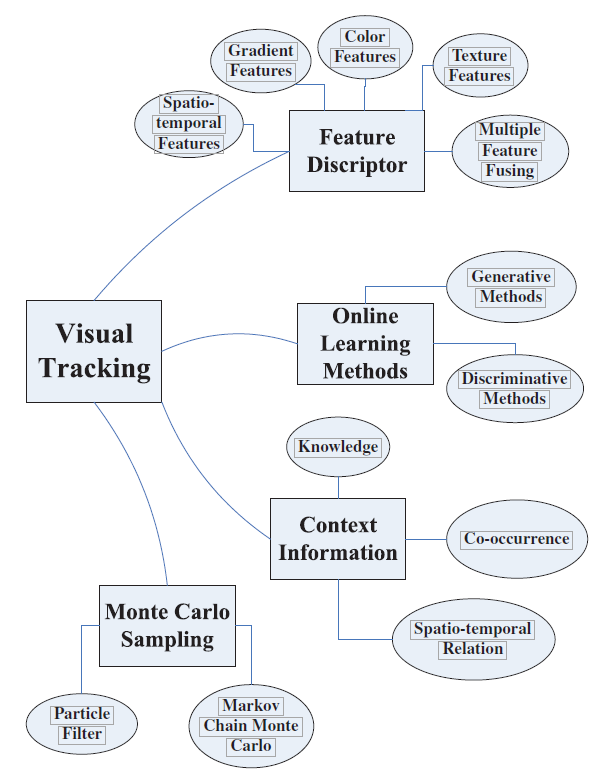
\includegraphics[width=0.45\linewidth]{figures/yang2011recent_graph.png}
   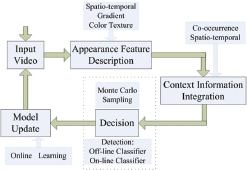
\includegraphics[width=0.45\linewidth]{figures/yang2011recent_flowchart.png}
   \caption{\textbf{Framework of tracking models}. From \cite{avidan2004support}.}
   \label{fig:yang2011recent}
\end{figure}


"State-of-the-art adaptive tracking-by-detection methods mainly
focus on improving tracking performance by increasing
the robustness of the classifier to poorly labelled samples
resulting from this approach. Examples of this include using
robust loss functions [6], [7], semi-supervised learning [8],
[9], or multiple-instance learning [3], [10]." \cite{hare2014struck}


% ====================
\section{Online RGB Trackers (vision papers)}
% ====================
Survey papers:
\begin{enumerate}
\item Yang et al. \cite{yang2011recent}. 2011 survey of the field
\item \textbf{Pang et al's Survey} \cite{pang2013finding} notes biases in
comparisons: usually new papers list their method as the best (because of a
specific methodology); however second best paper rankings are fairly robust. A
meta-analysis concludes the following methods are competitive: Struck, MIL, TLD,
VTD. 
\item \textbf{an extensive PAMI Survey} \cite{smeulders2013visual} claims Struck
is the best, and analyses specific failure cases and how it affects specific
method
\item \textbf{Appearance Model Survey} \cite{li2013survey}
\item A comprehensive list of papers can be found by searching papers that have
referenced Struck; which is the most frequently used benchmark to compare
against.
\item \textbf{Visual Tracking Benchmark}\cite{kristan2013visual} 
\item Wu et. al \cite{wu2013online} (SCM, Struck, TLD, ASLA, CXT, VTD, VTS, CSK)
concludes
    \begin{enumerate}
    \item \textbf{Background Information}  background
    information is critical for effective tracking. It can be ex-
    ploited by using advanced learning techniques to encode
    the background information in the discriminative model im-
    plicitly (e.g., Struck), or serving as the tracking contex-
    t explicitly (e.g., CXT)
    \item \textbf{local models}  are important for tracking as shown in the performance improvement of local sparse representation (e.g., ASLA and SCM) com-
    pared with the holistic sparse representation (e.g., MTT and
    L1APG). They are particularly useful when the appearance
    of target is partially changed, such as partial occlusion or
    deformation.
    \item \textbf{local models} motion model or dynamic model is cru-
    cial for object tracking, especially when the motion of target
    is large or abrupt. However, most of our evaluated tracker-
    s do not focus on this component. Good location predic-
    tion based on the dynamic model could reduce the search
    range and thus improve the tracking efficiency and robust-
    ness.
    \end{enumerate}
\item VOT2014 Results \cite{kristan2014visual}
\end{enumerate}

``The challenge considers single-camera, single-target, model-free, causal trackers, applied to short-term tracking. The model-free property means that the only supervised training example is provided by the bounding box in the first frame.  The short-term tracking means that the tracker does not perform re-detection after the target is lost. Drifting off the target is considered a failure. The causality means that the tracker does not use any future frames, or frames prior to re-initialization, to infer the object position in the current frame." \cite{kristan2014visual}

``In this paper, we focus on the problem of model-free online tracking of an object,
given only the object’s initial position and previous observations, within a tracking-bydetection
framework."\cite{zhang2014meem}

``Model drift occurs because factors like tracking failure, occlusions and misalignment
of training samples can lead to bad model updates. One remedy is to incorporate the first
frame template or prior knowledge in the online model update procedure [20,15]. However,
relying on a fixed model prior tends to restrict the tracker’s ability to handle large
object appearance changes. Other trackers [22,32,14] use a “censorship mechanism”
where an update is prevented when certain criteria are met (or not met). The detection
of good or bad updates usually relies upon smoothness assumptions for motion and
appearance changes, which are often violated in challenging scenarios. And once the
censorship mechanism fails, these trackers will either miss the chance to evolve or get
trapped in a background region, due to the fact that the model can only evolve forward,
without a mechanism to correct for past mistakes."\cite{zhang2014meem}

% --------------------
\subsection{Pre-CVPR 2013 Trackers}
% --------------------


\paragraph{Online RGB Trackers} require no prior knowledge of the object, and only a bounding box of the target on the original frame. 
A survey of tracking methods \cite{wu2013online} (SCM, Struck, TLD, ASLA, CXT, VTD, VTS, CSK), as well as papers following the survey \cite{supancic2013self}, show the following methods are competitive for this problem:
\begin{enumerate}
\item \textbf{Struck} \cite{hare2011struck}  uses a kernelized structured output SVM to directly learn displacement vectors. Gaussian kernel on 192 haar-like features. Struck's TPAMI paper \cite{hare2014struck}. 

Kernelization does most of the work, but structured SVM formulation avoids arbitrary hand-tuned parameters: "a large part of the performance gains... can be attributed to our use of a kernelised SVM rather than a boosting-based classifier."

``(previous) algorithms separate the adaptation phase of
the tracker into two distinct parts: (i) the generation and
labelling of samples; and (ii) the updating of the classifier."

``we make use of the structured output SVM
framework of Tsochantaridis et al. [15]. In particular, we
extend the online structured output SVM learning method
proposed by Bordes et al. [16], [17] and adapt it to the task
of adaptive object tracking."

\item \textbf{SCM} \cite{zhong2012robust} 
\item \textbf{TLD} \cite{kalal2012tracking} "We develop a novel learning method (P-N learning) which estimates the
errors by a pair of “experts”: (i) P-expert estimates missed detections, and (ii) N-expert estimates false alarms. The learning process is
modeled as a discrete dynamical system and the conditions under which the learning guarantees improvement are found. We describe
our real-time implementation of the TLD framework and the P-N learning.

\item \textbf{APG-L1} \cite{bao2012real} "l1 norm related minimization model".
\item \textbf{MIL} \cite{babenko2009visual} Older well-known tracker using multiple instance learning.
\item \textbf{CXT} \cite{dinh2011context} uses background context
\item \textbf{ASLA} \cite{jia2012visual} 
\item \textbf{Circulant} \cite{henriques2012exploiting} (TPAMI \cite{henriques2015tracking}) uses fourier transformed graham matrix to improve .

The fastest tracker in \cite{wu2013online}.

``a notable optimization
is to use a fast but inaccurate classifier to select promising
patches, and only apply the full, slower classifier on those
[18], [19]."

 


\item Zhang \cite{zhang2012real} "propose a projection to a fixed
random basis, to train a Naive Bayes classifier, inspired
by compressive sensing techniques."
\end{enumerate}


% --------------------
\subsection{Post-CVPR 2013 Trackers}
% --------------------
After Wu et. al's  survey \cite{wu2013online}, the following notable methods were also published:

\begin{enumerate}
\item \textbf{Self-paced learning} \cite{supancic2013self} "we show that an accurate appearance model is considerably more effective than a strong motion model". 
\item \textbf{MEEM} \cite{zhang2014meem} claims state-of-the-art over Struck, SCM, MIL.
\item \textbf{Xiang} \cite{xiang2014monocular}
\item \textbf{Occlusion and motion reasoning for long-term tracking} \cite{hua2014occlusion} "Struck fails in
the presence of long-term occlusions as well as severe viewpoint changes
of the object. In this paper we propose a principled way to combine occlusion and motion reasoning with a tracking-by-detection approach."
\item Color tracker \cite{danelljan2014adaptive} - the \textbf{best}.
\end{enumerate}

% --------------------
\subsection{Analysis}
% --------------------
Struck is a major paper, topping the benchmarks of Pang \cite{pang2013finding}, Wu \cite{wu2013online} and Smeulders \cite{smeulders2013visual}. Notably, newer papers aren't as well-tested and perhaps better. Struck is basically kernelized structured output SVMs, where $(x,y)$ are image patches and displacements. Most of the gains come from the kernelization, though.

Circulant trackers are really, quite good.



% =============================================
\section{Online RGB-D Trackers (vision papers)}
\label{sec:online}
% =============================================
\paragraph{Online RGB-D Trackers} no prior knowledge of the object.
Song et. al's survey \cite{song2013tracking}, show \textbf{incorporating depth into tracking beats the state of the art.} It shows \textbf{Struck} \cite{hare2011struck} and VTD are competitive.

\textbf{Gaussian Process Regression} \cite{gao2014transfer} beats struck and Song et. al's survey benchmarks.

% =============================================
\section{Trackers (robotics papers)}
\label{sec:trackers}
% =============================================
\begin{enumerate}
\item RSS 14: Anytime Tracking \cite{held2014combining}
\item RSS 14: DART Pose Estimation \cite{schmidt2014dart} (relevant?)
\item ICRA: Small Obstacle Discovery over Images \cite{kumar2014markov}: small object segmentation using RGB, since depth info doesn't give much.
\item ICRA 14: Tracking ping pong balls \cite{zhang2014spin} This paper proposes a way to observe and estimate ball's spin in real-time, and achieve an accurate prediction. Based on the fact that a spinning ball's motion can be separated into global movement and spinning respect to its center, we construct an integrated vision system to observe the two motions separately. With a pan-tilt vision system, the spinning motion is observed through recognizing the position of the brand on the ball and restoring the 3D pose of the ball. Then the spin state is estimated with the method of plane fitting on current and historical observations. With both position and spin information, accurate state estimation and trajectory prediction are realized via Extended Kalman Filter(EKF). 
\item ICRA 14: road scene segmentation \cite{huang2014road} "we first produce initial object hypotheses by clustering the sparse 3D point cloud. The image pixels registered to the clustered 3D points are taken as samples to learn each object's prior knowledge. The priors are represented by Gaussian Mixture Models (GMMs) of color and 3D location information only, requiring no high-level features. We further formulate the segmentation problem within a Conditional Random Field (CRF) framework, which incorporates the learned prior models, together with hard constraints placed on the registered pixels and pairwise spatial constraints to achieve final results. "
\item ICRA 14: Learning latent structure for activity recognition \cite{hu2014learning}. Good overview of basics.
\end{enumerate}
% =============================================
\section{Temporal Speech Data}
\label{sec:temporalspeech}
% =============================================
Structured prediction is used in temporal data such as speech recognition. This
has yet to fully permeate object tracking in videos.

RGB-D videos provide a unique set of data to images. Objects are more easily
segmented based on depth data (without transformation) alone. This can be seen
in LIDAR \cite{morton2013multi}.

It is often the case that 


% =============================================
\section{RGB-D Datasets}
% =============================================
\begin{enumerate}
\item Princeton RGB-D \cite{song2013tracking}
\item Wu et al. \cite{wu2013online}
\item Bigbird \cite{singh2014bigbird} (relevant?)
\end{enumerate}
% =============================================
\section{RGB-D Features}
% =============================================
\begin{enumerate}
\item Learning rich features from rgb-d images for object detection and segmentation \cite{gupta2014learning}
\item Segmentation using RGB-D data \cite{abramov2012depth}
\item Shotton's Random Forest \cite{shotton2013real}: ``each feature need only
read at most 3 image pixels and perform at most 5 arithmetic
operations; and the features can be straightforwardly implemented
on the GPU. Given a larger computational budget,
one could employ potentially more powerful features based
on, for example, depth integrals over regions, curvature, or
local descriptors"

\begin{figure}
   \hspace{-2mm}
   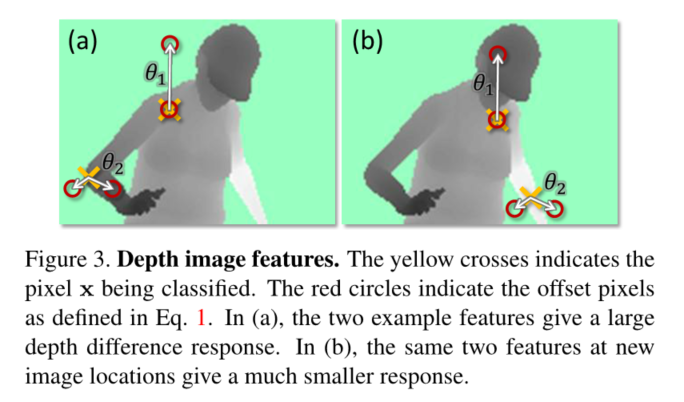
\includegraphics[width=0.45\linewidth]{figures/shotton2013real_features.png}
   \caption{\textbf{Shotton's Random Forest} \cite{shotton2013real}}
   \label{fig:shotton2013real_features}
\end{figure}
\end{enumerate}

% =============================================
\subsection{Shotton Random Forests}
% =============================================

% ====================
\section{Early Tracking}
% ====================
Tracking pre-2005ish.

CONDENSATION—Conditional Density Propagation for Visual Tracking: "The problem of tracking curves in dense visual clutter is challenging. Kalman filtering is inadequate because it is based on Gaussian densities which, being unimodal, cannot represent simultaneous alternative hypotheses. The CONDENSATION algorithm uses ``factored sampling'', previously applied to the interpretation of static images, in which the probability distribution of possible interpretations is represented by a randomly generated set. CONDENSATION uses learned dynamical models, together with visual observations, to propagate the random set over time. The result is highly robust tracking of agile motion. Notwithstanding the use of stochastic methods, the algorithm runs in near real-time."

http://www.cse.psu.edu/~rcollins/CollinsVLPR2012Lecture.pdf
http://www.cse.psu.edu/~rcollins/CollinsVLPR2009Lecture.pdf

% ====================
\section{Misc Other things}
% ====================

Pedestrian detection using optical flow. \cite{benenson2014ten}

\textbf{FABMAP}:
Bag of words,  descriptor, vector quantization into a visual word, Chow-liu trees for bayesian probability

% ====================
\section{Techniques}
% ====================
\begin{enumerate}
\item Structured SVMs: vedaldi2014structuredsvm
\item Multi-resolution \cite{park2010multiresolution}: for finite resolution cameras, scale variance is needed.
\end{enumerate}

% ====================
\section{Other Techniques}
% ====================
Gaussian Processes Bible (with matlab toolbox) \cite{rasmussen2006gaussian}
% --------------------

% --------------------
% ====================
\chapter{Method (My Idea)}
% ====================

% • In a paper you MUST provide the details, but FIRST convey the idea
% • Introduce the problem, and your idea, using EXAMPLES and only then
% present the general case
% • Explain it as if you were speaking to someone using a whiteboard
% • Conveying the intuition is primary, not secondary
% • Once your reader has the intuition, she can follow the details (but not vice
% versa)
% Even if she skips the details, she still takes away something valuable
% Evidence
% • Your introduction makes claims; The body of the paper provides evidence to
% support each claim
% • Check each claim in the introduction, identify the evidence, and forward-
% reference it from the claim
% • Evidence can be: analysis and comparison, theorems, measurements, case
% studies

% ====================
\section{My Idea (2 pages)}
% ====================

% ====================
\section{The details (5 pages)}
% ====================

% ====================
\chapter{Motion Planning}
% ====================
% --------------------
\section{Basic Ingredients}
% --------------------
\begin{itemize}
\item State
\item Time
\item Actions
\item Initial and Goal States
\item Feasibility and Optimality Criterion
\item A Plan
\end{itemize}

For a full description, see Chapter 1.3 of Lavalle \cite{lavalle2006planning}.
% --------------------
\section{Introduction to Motion Planning}
% --------------------
% --------------------
\subsection{Simple Motion Planning}
% --------------------
The simplest motion planning problems assume knowledge of a global map, a fixed
known goal state and a fixed known initial state. The problem is to determine a
feasible path from the initial state to the goal state. An optimality criterion
may also be applied to choose the best path if multiple feasible ones are found.

Notably, two important concepts have often been ignored in determining the path:
the dynamics of the system and the use of feedback. Dynamics refers to how
states transition to other states, and is inherent in real-world systems. For
example, a car can easily move fowards and backwards, but cannot immediately
move side to side. Feedback refers to the technique of refining further actions
based on newly sensed data. In simulations, feedback may not be necessary, but
in real-world systems, errors in sensing and modeling build up over time without
it.

In this simple case, the generated path is followed in an open-loop manner, or
if subject to real-world constraints (see \autoref{fig:lavalle2006planning119}),
the generated path is smoothed to obey the system's dynamics and feedback is
used to closely follow the path. "Notably this approach is highly decoupled as
feedback and dynamics are neglected in constructing the original path"
\cite{lavalle2006planning}. The smooth path may now obey the robot's dynamics,
but may no longer be feasible.  Feedback is used merely as an inefficient
afterthought.

\begin{figure}
\centering
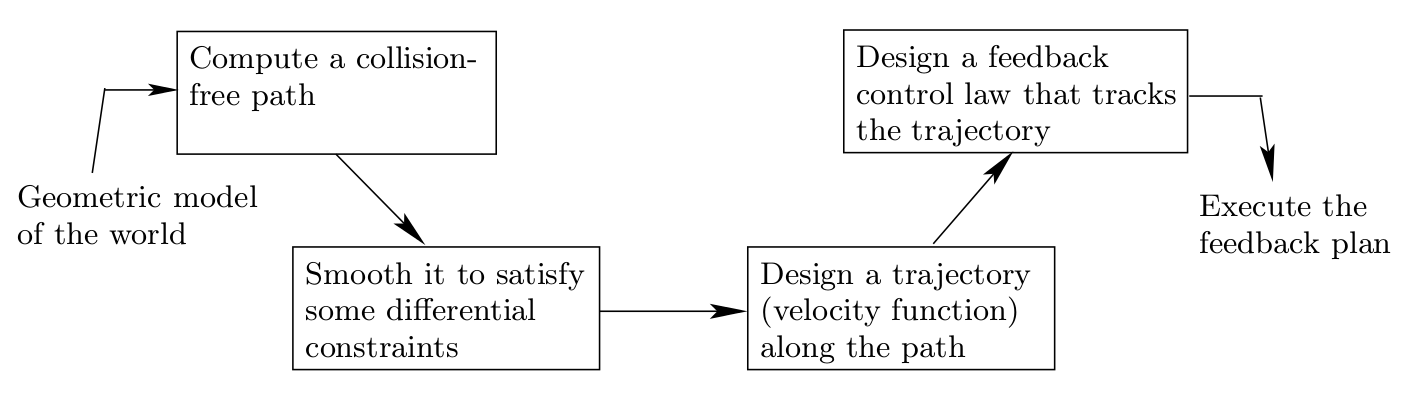
\includegraphics[width=3in]{figures/lavalle2006planning119.png}
\caption{From \cite{lavalle2006planning}. A refinement approach that has been used for decades in robotics.}
\label{fig:lavalle2006planning119}
\end{figure}

Even in this simple case, obtaining an optimal or even feasible path is not
straightforward if the state space is large. A* search for trivially sized state
spaces and sampling-based techniques such as RRTs (RRT* for optimality) and PRMs
have proven to be the methods of choice (citation?), though it is still an
ongoing field of interest (cite 2015 RRT/PRM papers).

% --------------------
\subsection{Feedback Motion Planning}
% --------------------
Dynamics refers, generally, to how a state transitions to another state.

Feedback (or reactive plans) refers to something else.

Tiers of motion planning problems
\begin{itemize}
\item Fixed Initial and Goal States, no dynamics, no feedback, some optimality
criterion: RRT*, PRM*
\item Fixed Initial and Goal States, dynamics, no feedback: RRT*, A*
\item Fixed Initial and Goal States, no dynamics, feedback
\end{itemize}

see \autoref{fig:determinedrive2}.
\begin{figure}
\centering
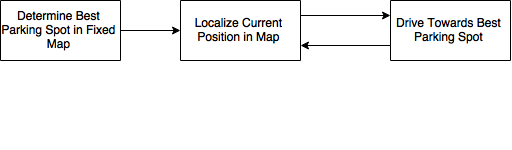
\includegraphics[width=3in]{figures/determinedrive2.png}
\caption{Feedback loop}
\label{fig:determinedrive2}
\end{figure}


% --------------------
\subsection{Feedback Motion Planning with Updating Goal State}
% --------------------
see \autoref{fig:determinedrive1}.
For a full description, see Chapter 8 of Lavalle \cite{lavalle2006planning}.

\begin{figure}
\centering
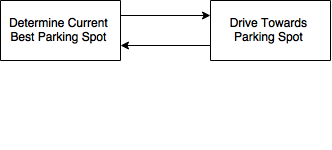
\includegraphics[width=3in]{figures/determinedrive1.png}
\caption{Feedback loop}
\label{fig:determinedrive1}
\end{figure}


% --------------------

% --------------------
\chapter{Experiments}
\label{ch:experiments}


% ====================
\section{Installing F}
% ====================

\begin{enumerate}
	\item implement princeton RGBD algorithm
	\item implement struck
	\item implement 2014 color tracking algorithm
	\item implemenmt Gaussian processes algorithm
\end{enumerate}

\subsubsection{Implementing the princeton "song2013tracking" RBGD algorith}

code is in song2013tracking. 

% --------------------



%\include{model}
%\include{impl}
%\include{discussion}
%\include{conclusions}

%    3. Notes
%    4. Footnotes

% --------------------
%    5. Bibliography
% --------------------
\begin{singlespace}
\raggedright
\bibliographystyle{abbrvnat}
\bibliography{biblio}
\end{singlespace}

% --------------------
\appendix
%    6. Appendices (including copies of all required UBC Research
%       Ethics Board's Certificates of Approval)
%\include{reb-coa}	% pdfpages is useful here
% --------------------
\chapter{Supporting Materials}

This would be any supporting material not central to the dissertation.
For example:
\begin{itemize}
\item additional details of methodology and/or data;
\item diagrams of specialized equipment developed.;
\item copies of questionnaires and survey instruments.
\end{itemize}


% --------------------
\backmatter
%    7. Index
% See the makeindex package: the following page provides a quick overview
% <http://www.image.ufl.edu/help/latex/latex_indexes.shtml>
% --------------------


\end{document}
